\section{Introduction}

 The goal of our programming project is about developing a Python-based GUI (Graphical User Interface) that interfaces PyTorch; an open-source deep learning frameworks.
 \newline Like Expresso for Caffe, NVidia DIGITS for Theano, Caffe, Torch and Tensorflow. A lot of graphical user interface which provide numerous tools for deep learning frameworks are available. Unfortunately they are not compatible with the PyTorch Library at the time when we begin this project. So, the alternative we propose is an application that will be an interface for PyTorch and gives the abilities to use all the deep learning features provided by the Pytorch framework.
 \newline Our application goal is to provides interesting features with manipulation of neural network. It will also integrate Jupyter-Notebook thus user could expereience live coding, graph computation and specifically neural network vizualisations. 


\begin{figure}[!ht]
    \center
    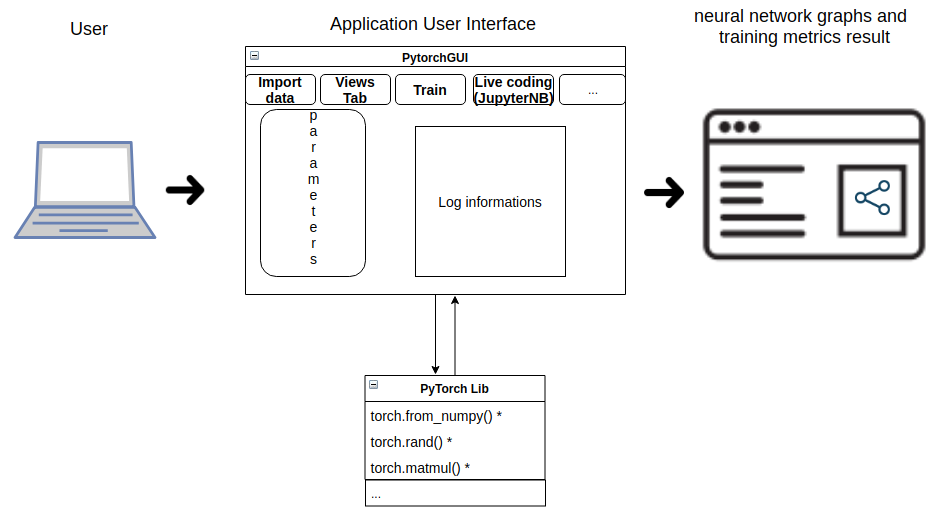
\includegraphics[scale=0.4]{figures/schema_intro1.png}
    \caption{Schematic view of the project}
\end{figure}
\footnote{Features shown in this schema will be discuss further below}

\section{Definitions}
Before we dive in the project code implementation and it's architecture let us start with some fundamentals in Artificial Intelligence and examples.

\subsection{Artificial Intelligence, Machine learning and Deep Learning}
In the early days, of AI, algorithms were used to solve problems that where difficult for humans to solve. Machine were hard coded, such as a computer program playing chess.
\newline Machine learning is one of the fields of study of Artificial Intelligence. It relies on statistical concepts as well as models to give machines the ability to learn. It basically consists of showing a lots of examples, using a set of data, the training set, to make our algorithm try to recognize patterns in it, so it can learn to recognize new data instantly thus come up with rules to predict outcomes for unseen data:

\begin{figure}[!ht]
    \center
    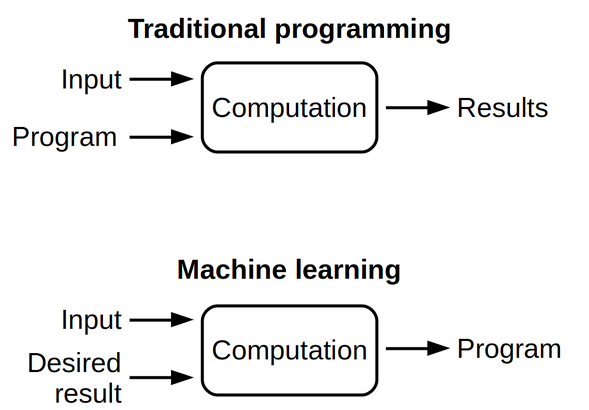
\includegraphics[scale=0.3]{figures/marchine_learning_para.png}
    \caption{Traditional Programming vs Machine Learning}
\end{figure}


The training phase of a machine learning algorithm takes the training set, and tries for a pre-determined number of iterations, to classify the data. In each iteration, the algorithm will take into account the errors of classification in the last iteration to correct itself, step by step, until its accuracy is high enough.

There are different types of approach for machine learning algorithms :
\begin{itemize}
\item Supervised learning : In this case, the data is annotated, which means the algorithm knows the inputs and the outputs of the set. It allows to directly check if the result is correct in each iteration.
\item Semi-supervised learning : In this case it's the same as supervised learning, with the exception that only a part of the data is annotated
\item Unsupervised learning : This type of approach is clearly distinct from the two others, since the data is not annotated. In this case, the algorithm will try to find patterns by itself, without the use of external corrections. It's only after training that the user can see the results.
\end{itemize}

Once the training of the algorithm is finished, we can evaluate it by using another data-set, which contains different data than the training set, to evaluate the accuracy of our algorithm. \usetikzlibrary{}Here is a visualization among AI, ML and DL.

\begin{figure}[!ht]
    \center
    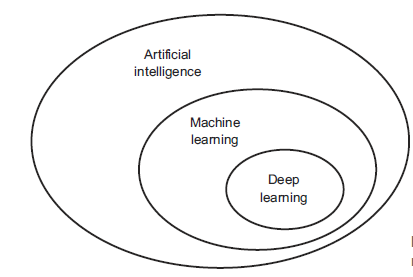
\includegraphics[scale=0.5]{figures/aivsmlvsdl.png}
    \caption{About AI}
\end{figure}

Deep Learning algorithms are a part of the machine learning family algorithms. To be able to recognize patterns in data, they use a cascade of multiple layers of nonlinear processing units. Each layer uses the output from the previous one. They work with the concept of deep neural networks.

\newpage
\subsection{PyTorch}
In Pytorch, data are represented as tensor or variable.
\subsubsection{Tensor}
Tensor are Python's numpy array but they can be used with GPU. In our project we will not use the GPU but the CPU, we still working on this feature it will be avaible in newer version of the app. But tensor still useable with CPUs. 
\newline Like arrays, tensors contains elements and can be multidimensional. Frequenntly used tensor are :
\begin{itemize}
    \item Scalar (0-D tensors)
    \item Vector (1-D tensors)
    \item Matrix (2-D tensors)
    \item 3-D tensors
    \item Slicing - tensors
    \item 4-D tensors
    \item 5-D tensors
\end{itemize}

For example, image can be represented as 3D-Tensor (height,weight, channel (RGB)) so a 4D-Tensor can be a Tensor with a batch of images. The number of images are represented in the 4th dimension. Slicing tensor are one-dimensional tensor that we slice the elements. For example 1-D\_tensor\textit{[:slice\_index]}   

\subsubsection{Variables}
Pytorch variables can be seen as containers with:
\begin{itemize}
    \item Data : tensor object
    \item Gradients
    \item Creator: reference to the function that created it
\end{itemize}

\subsection{Computation graphs}
To represent deep learning algorithms we can use graphs. The following computational graph computes the sum z of two inputs x and y:

\begin{figure}[!ht]
    \center
    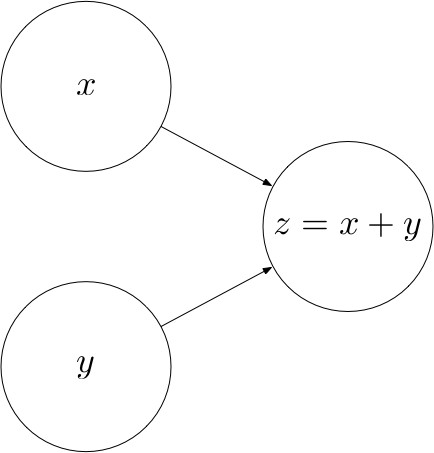
\includegraphics[scale=0.4]{figures/computational_graph.png}
    \caption{Representation of a computational graph }
\end{figure}

Here, x and y are input nodes to z and z is a consumer of x and y. 
\subsection{Neural network model}
To build a model wich learns how to map the outputs from the inputs we must learn the network (functoin) by showing the inputs and the associated output. For a linear relationship model represented as y = wx + b. Here is its associated computation graph:

\begin{figure}[!ht]
    \center
    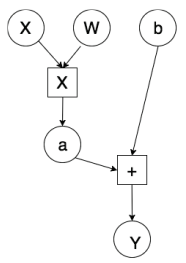
\includegraphics[scale=0.8]{figures/linear.png}
    \caption{Linear relationship graph }
\end{figure}

\subsubsection{implementation}
\begin{lstlisting}
def linear_model(x):
    y = torch.matmul(x,w)
    return y
\end{lstlisting}

\subsection{Layer}
\subsubsection{torch.nn}
Pytorch provides a higher level abstraction in torch.nn called layers wich create latyer much simpler.
\begin{lstlisting}
class torch.nn.Linear(in_features, out_features, bias=True)
\end{lstlisting}
Applies a linear transformation to the incoming data: y=Ax+b
\newline Parameters:	
\begin{itemize}
    \item in\_features – size of each input sample
    \item out\_features – size of each output sample
    \item bias – If set to False, the layer will not learn an additive bias. Default: True
\end{itemize}

\noindent The previous model can be represented as a torch.nn layer as follow:
    \begin{lstlisting}
    f = nn.Linear(17,1) 
    \end{lstlisting}

\subsection{Loss function}
